\chapter{Experiments and results}
\label{AER}


\section{Forecasting skill}
In this section we evaluate the general forecasting skill for our model. Tables \ref{tab:MSE_31}-\ref{tab:MSE_127} show the MSE for different variables across lead times for each grid resolution. To Enable per variable comparison, we plot heatmaps of these results per variable across grid resolutions and lead times, shown in Figures \ref{fig:heatmap_temp}-\ref{fig:heatmap_vor} across different lead times and three vertical levels. 

The prediction skill for temperature, shown in Figure \ref{fig:heatmap_temp}, demonstrates that increasing prediction lead time generally leads to a degradation in predictive performance. This is expected, as the atmosphere is a highly chaotic system where errors accumulate non-linearly over time. This pattern of temporal degradation is consistent across all variables, including geopotential and vorticity, as shown in Figures \ref{fig:heatmap_geopot} and \ref{fig:heatmap_vor}.

When examining the effect of grid resolution on temperature forecasting, we observe a non-monotonic relationship. At short lead times (6h), there is a clear improvement in MSE as resolution increases from TL31 (5.86) to TL95 (4.30). This suggests that the added expressivity of the closure term, described in Section \ref{sec:gnn_scaling}, successfully recovers unresolved scales of temperature dynamics. However, as lead time increases, the coarsest grid (TL31) produces the lowest MSE (9.51 at 1~d vs. 12.19 for TL127). This inversion is likely because the coarser grid acts as a low-pass filter, suppressing high-frequency, unpredictable scales that diverge rapidly due to chaotic error growth. Furthermore, the lower resolution minimizes the `double penalty' effect inherent in MSE metrics, where sharper, high-resolution features that are slightly spatially displaced are penalized more heavily than smooth, coarse-resolution fields.

The effect of grid resolution on geopotential and vorticity is more heterogeneous and highlights a specific limitation at the highest resolutions. Surprisingly, for both variables, the highest resolution grid (TL127) often provided the poorest performance. For geopotential at 500~hPa (1~d lead time), the TL127 grid yielded an MSE of $2.92 \times 10^7$, significantly higher than the TL95 grid ($1.24 \times 10^7$) and even the coarse TL31 grid ($1.28 \times 10^7$). Similarly, for vorticity at 850~hPa (6h lead time), the TL127 error ($1.10 \times 10^{-9}$) was nearly double that of the TL63 grid ($6.21 \times 10^{-10}$), which acted as a performance ``sweet spot.''

This degradation at TL127 may be linked to the resolution-aware scaling of the GNN architecture detailed in Section \ref{sec:gnn_scaling}. To maintain computational efficiency, the hidden layer width $d$ was scaled inversely with the square root of the number of grid nodes ($d_{127} = 64$ vs. $d_{31} = 256$). While this keeps the total compute budget comparable, the reduced per-node capacity at TL127 may limit the closure's ability to capture complex sub-grid interactions at fine scales, potentially rendering the solver more susceptible to high-wavenumber noise.

Divergence follows a trend strongly favoring lower resolutions. As shown in Figure \ref{fig:heatmap_div}, the coarsest grid (TL31) consistently outperformed finer grids. At 500~hPa, the TL31 grid maintained an MSE of $1.69 \times 10^{-10}$ at the 6h mark, compared to $2.51 \times 10^{-10}$ for TL127. This suggests that divergence is particularly sensitive to small-scale noise, which is effectively filtered out by the coarser discretization.

In contrast, specific humidity displays a clearer benefit from increased resolution, though it remains subject to the TL127 degradation. Unlike dynamical variables where TL31 often excelled, specific humidity prediction suffered at the coarsest resolution ($2.40 \times 10^{-5}$ at 500~hPa, 6h). The finer TL95 grid reduced this error significantly to $5.45 \times 10^{-6}$, indicating that moisture dynamics rely heavily on resolving localized, small-scale features. However, at TL127, the error rose again to $1.16 \times 10^{-5}$, reinforcing the observation that while fine-scale resolution is necessary for moisture, the highest resolution configuration (TL127) struggles to balance error growth and correction capacity.


\begin{figure}
    \centering
    
\includegraphics[width=0.99\linewidth]{Figures/mse_heatmap_byvar_temperature_6h12h1d.pdf}
    \caption{MSE across lead times and grid resolutions for temperature}
    \label{fig:heatmap_temp}
\end{figure}


\begin{figure}
    \centering
    
\includegraphics[trim=5 5 5 15,clip,width=0.99\linewidth]{Figures/mse_heatmap_byvar_geopotential_6h12h1d.pdf}
    \caption{MSE across lead times and grid resolutions for geopotential}
    \label{fig:heatmap_geopot}
\end{figure}

\begin{figure}
    \centering
    
\includegraphics[width=0.99\linewidth]{Figures/mse_heatmap_byvar_vorticity_6h12h1d.pdf}
    \caption{MSE across lead times and grid resolutions for vorticity}
    \label{fig:heatmap_vor}
\end{figure}

\begin{figure}
    \centering
    
\includegraphics[width=0.99\linewidth]{Figures/mse_heatmap_byvar_divergence_6h12h1d.pdf}
    \caption{MSE across lead times and grid resolutions for divergence}
    \label{fig:heatmap_div}
\end{figure}

\begin{figure}
    \centering
    \includegraphics[width=0.99\linewidth]{Figures/geopotential_850hPa_init_2020-01-02T00_models.pdf}
    \caption{Forecasting skill visualisations across different lead times for geopotential at 850\,hPa initialised at \(2020\text{-}01\text{-}01 \; \mathrm{T}00:00\). Columns show lead times \(+6\)h, \(+12\)h, and \(+48\)h; rows compare the ERA5 target (Truth), the hybrid forecast (Prediction), the dynamical core alone (Dycore), and the learned correction component (GNN correction). The bottom panels report residuals (Prediction$-$Truth). All fields are shown on the TL127 evaluation grid (units: K).}
    \label{fig:skill_visuals_crosslead:geopot}
\end{figure}

\begin{figure}
    \centering
    \includegraphics[width=0.99\linewidth]{Figures/temperature_850hPa_init_2020-01-02T00_models.pdf}
    \caption{Forecasting skill visualisations across different grid types for temperature at 850\,hPa initialised at \(2020\text{-}01\text{-}01 \; \mathrm{T}00:00\). Columns show grid types; rows compare the ERA5 target (Truth), the hybrid forecast (Prediction), the dynamical core alone (Dycore), and the learned correction component (GNN correction). The bottom panels report residuals (Prediction$-$Truth). All fields are shown on the TL127 evaluation grid (units: K).}
    \label{fig:skill_visuals_crossgrid:temperature}
\end{figure}

\section{Spectral cross-scale analysis}

\subsection{Energy Spectrum}
A common way to quantify the quality of forecasting models is to compare their energy spectra to the ground truth. This allows for the evaluation of the models "blurriness", so how well the model capture high frequency variation of the predicted fields. Fig

\subsection{Closure gain}
As one of the main contributions of the thesis, we presents the results of the closure gain experiment in Figures \ref{fig:gain_wavenumbers}-\ref{fig:gain_TL47_leadtimes}. The aim of these experiments was to better characterize the interactions of the two model components (numerical core and learned Closure), using the linearised gain metrics $f^{+}$ and $f^{-}$ defined in Section \ref{sec:gain-experiment}. To achieve more general observations, the results presented in this section were calculated from the ensemble of all reference states included in the test set. This meant all corresponding to the $6$-hourly init times for the year $2020$, totalling in $N=1464$ reference states.

Overall, gain values are mostly above $1$, which means the closure is in general amplifying dycore tendencies. This suggests that, in the linearised sense of Section~\ref{sec:gain-experiment}, the learned closure provides a predominantly \emph{positive feedback} along many spherical–harmonic directions, partially counteracting the net damping introduced by truncation, filtering, and implicit/numerical diffusion in the spectral core.

\subsection{The effect of lead time}
We examine how increasing the prediction lead time affects the closure gain. Figures~\ref{fig:gain_TL47_leadtimes}--\ref{fig:gain_TL127_leadtimes} show how the fraction of amplifying modes (\(\bar{g}_\ell > 1\)) and damping modes (\(\bar{g}_\ell < 1\)) changes with lead time for truncations TL47, TL95, and TL127. Across all grids, the fraction of amplifying modes decreases as lead time increases, while the fraction of damping modes increases.

A likely explanation is the well-known \emph{over-smoothing} phenomenon in learned chaotic dynamical systems: as the rollout horizon grows, small errors amplify, and the training objective increasingly penalizes sharp gradients and strongly unstable dynamics. Models therefore tend to converge toward smoother, less energetic evolution. In our setting, this manifests as the learned closure becoming more dissipative at longer lead times (more \(\bar{g}_\ell < 1\)) and less frequently reinforcing the dynamical-core tendencies (fewer \(\bar{g}_\ell > 1\)). We note that the fraction of modes with approximately unchanged tendencies (\(\bar{g}_\ell \approx 1\)) is very small (\(\ll 1\%\)) and is therefore omitted from the plots.

Interestingly, none of the metrics varies linearly with lead time; instead, they exhibit a knee-like, piecewise trend whose shape depends on grid resolution. The transition points occur at different lead times for different truncations. This behavior is unlikely to be a direct artefact of rollout training, since the rollout checkpoints were fixed at $[1, 2, 3, 4, 6, 8, 10]$ across all resolutions. We further discuss possible explanations in Chapter~\ref{Discussion}.


\subsubsection{Gain spectral distribution}

When examining the spectral distribution of the gain (Figure~\ref{fig:gain_wavenumbers}), we can make several observations. In general, $\flneg$ is highest at low wavenumbers and lowest at high wavenumbers, while the opposite is true for $\flpos$. This indicates that the learned closure is comparatively more dissipative on the largest resolved scales (small $\ell$), whereas it more frequently reinforces the dynamical--core tendencies on smaller spatial scales (large $\ell$). One plausible interpretation is that the closure primarily acts to maintain small-scale variability that is otherwise attenuated by the numerical core, while providing additional stabilisation on the slowly evolving, large-scale components of the flow. For instance, imagine a weather map with a big, smooth warm region covering half a country (large scale) and a few sharp storm lines or rain bands on top of it (small scale). The numerical core and its filtering tend to smooth out those sharp rain bands, so the closure “boosts” the small-scale features to keep them visible, while slightly damping the large-scale background to avoid the whole pattern drifting or oscillating unrealistically.

Another notable feature is a clear and pronounced dip in $\flneg$ and a corresponding increase in $\flpos$ near the eighth decile of the representable wavenumbers. This behaviour is a direct and expected consequence of the spectral filtering applied in the dynamical core. As discussed in Section~\ref{subsec:filtering}, spectral filtering is used to suppress spurious small-scale variance and prevent numerical instabilities associated with poorly resolved, fast dynamics. The learned GNN closure then partially compensates for this artificial damping by restoring variability at the affected scales, which manifests as increased amplification at high wavenumbers. Interestingly, although the filter attenuates the highest wavenumbers most strongly, we observe a renewed increase in the fraction of damping modes very close to the truncation limit. A plausible explanation is an end-of-spectrum artefact, such as aliasing and quadrature/transform errors near the highest retained modes, which can bias diagnostics at the grid scale. Consistent with this interpretation, the effect is more pronounced at lower resolutions, where the top-of-spectrum band contains fewer modes and is therefore more sensitive to discretisation and binning effects.

In general, lower-resolution grids exhibit a larger fraction of normalised-wavenumber gains below 1, especially at longer lead times and at lower normalised wavenumbers. This is attributed to the stronger effective dissipation and reduced scale separation at coarse resolution, where truncated nonlinear interactions and numerical filtering damp variability more aggressively. Consequently, the closure behaves more diffusively to stabilise the rollout, whereas at higher resolution it can preserve (or restore) a larger share of the resolved-scale variance.

\begin{figure}
    \centering
    
\includegraphics[width=0.8\linewidth]{Figures/curves_pr_damp_vs_knorm__lead_bins.pdf}
    \caption{Correction (closure) spectral gain fractions vs normalised wavenumber across for grid resolutions TL31 vs TL127. Column shows the spectral gains distribution on the early ($t=6h-36h]$), the mid ($t=42h-62h$) and the late ($t=[12,18]$ timepoints.}
    \label{fig:gain_wavenumbers}
\end{figure}

\begin{figure}
    \centering
    
\includegraphics[width=0.7\linewidth]{Figures/heatmap_lead_k__TL95__ohuef1pm.pdf}
    \caption{Dampening vs Amplifiying across different lead times for TL95.}
    \label{fig:gain_TL95_heatmap}
\end{figure}

\begin{figure}
    \centering
    
\includegraphics[width=0.7\linewidth]{Figures/heatmap_lead_k__TL47__thn1drla.pdf}
    \caption{Dampening vs Amplifiying across different lead times for TL47.}
    \label{fig:gain_TL47_heatmap}
\end{figure}

\begin{figure}
    \centering
    
\includegraphics[width=0.7\linewidth]{Figures/lead_summary__TL95__ohuef1pm.pdf}
    \caption{Gain statistics for different lead times for TL95.}
    \label{fig:gain_TL95_leadtimes}
\end{figure}

\begin{figure}
    \centering
    
\includegraphics[width=0.7\linewidth]{Figures/lead_summary__TL127__z87avopm.pdf}
    \caption{Gain statistics for different lead times for TL127.}
    \label{fig:gain_TL127_leadtimes}
\end{figure}

\begin{figure}
    \centering
    
\includegraphics[width=0.7\linewidth]{Figures/lead_summary__TL47__thn1drla.pdf}
    \caption{Gain statistics for different lead times for TL47.}
    \label{fig:gain_TL47_leadtimes}
\end{figure}

\section{Ablation studies}

To experimentally validate the architectural and training choices of our model, we conducted multiple ablation studies, notably: the choice of a hybrid architecture, and the choice of training for longer autoregressive rollouts.

\subsection{ML Only and Numerical Only}

One of the main justifications of our hybrid architecture is the improved data efficiency of such models compared to purely neural counterparts. To test this in practice, we implemented an ML-only and a dycore-only variant of our model.

In the ML-only variant, the dynamical core is removed entirely and the neural network is responsible for predicting the complete time evolution of the atmospheric state. Since neither the explicit resolved tendency $\mathcal{R}^{\mathrm{exp}}$ nor the implicit resolved tendency $\mathcal{R}^{\mathrm{imp}}$ is present, the IMEX scheme of Eq.~\eqref{eq:imex} reduces to a forward Euler update:
\begin{equation}
    \widetilde{g}^{\,n+1} = \widetilde{g}^{\,n} + \Delta t \;\operatorname{nn}_\theta\!\bigl(\widetilde{g}^{\,n},\mu\bigr),
    \label{eq:ml_only_update}
\end{equation}
where $\operatorname{nn}_\theta$ now predicts the full tendency without any dynamical-core contribution.

Similarly, the dycore-only variant does not incorporate the contributions of the learned correction; it reduces to a regular spectral numerical solver advanced with the same IMEX scheme as the hybrid model (Eq.~\eqref{eq:imex}), but with $\operatorname{nn}_\theta \equiv 0$.

Table~\ref{tab:ablation_ml_dycore_only} shows the results of the ablation study for a 6~h prediction range. The hybrid architecture has a clear advantage over the ML-only and dycore-only variants, which highlights the effectiveness of the approach. Notably, the hybrid variant outperforms the ML-only variant trained on $12$K data points after seeing only $\sim\!1900$ data points, demonstrating the improved data efficiency afforded by the physics priors incorporated into the numerical solver.




\begin{table}[ht]
\centering
\small
\begin{tabular}{lccc}
\hline
\textbf{Level (hPa)} & \textbf{Dycore only} & \textbf{GNN only} & \textbf{Hybrid} \\
\hline\hline
500 & 46.1 & 11.1 & \textbf{4.55} \\
700 & 36.7 & 8.8 & \textbf{3.62} \\
850 & 57.4 & 13.9 & \textbf{5.67} \\
\hline
\end{tabular}
\caption{Comparison of hybrid vs non-hybrid variants of the model: The table shows the test MSE for the temperature variable at 6h lead time for TL127 resolution across model variants. The best result in each row is in bold.}
\label{tab:ablation_ml_dycore_only}
\end{table}

\subsection{Rollout trainings}

As discussed in Section \ref{sec:formal_closure}, there are multiple approaches to neural closure modelling, depending on how the reduced scale (resolved) model is incorporated. To assess the difference between the two discussed approaches, we conducted an ablation study comparing offline and online training regimes.

In our setup, \textit{offline} (or \textit{a priori}) training corresponds to training the model for a single inference step (6 hours). This is termed ``offline'' because the closure is optimized to minimize the immediate error against a fixed ground truth target at $t+1$, without feeding the prediction back into the solver. Conversely, \textit{online} (or \textit{a posteriori}) learning corresponds to fitting entire trajectories, where the differentiable solver is unrolled for multiple autoregressive steps (24 hours in this experiment) and the loss is calculated over the full path. This setup means the predictions are fed back into the model, thus the dynamical effects of model predictions made at $t$ are incorporated into the model evaluation at $t+\delta t$.

To ensure a fair comparison, the total number of training data points was matched across the two regimes; the online approach processes data in trajectory blocks, while the offline approach processes an equivalent number of independent snapshots, ensuring neither model benefits from additional data volume. The results, shown in Figure \ref{fig:rmse_horizon} (see Figure 4.11), confirm the effectiveness of training on longer rollouts. The online (24h) trained model consistently outperforms the offline (6h) variant. Notably, this performance gain is observed even for the single-step (6h) inference, and the advantage grows significantly as the forecast horizon extends to 30 hours.


\begin{figure}
    \centering
    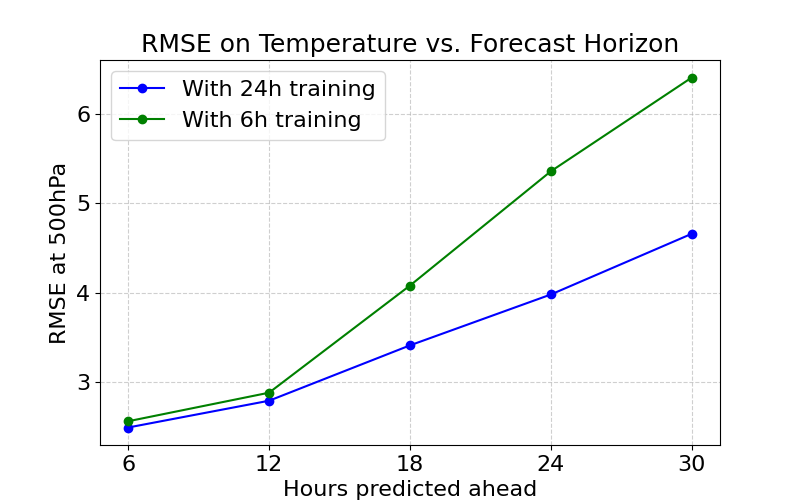
\includegraphics[width=0.7\linewidth]{Figures/Matched_rmse.png}
    \caption{Empirical evaluation of different closure modelling approaches and their corresponding training regimes. "With 6 hour training" corresponds to the \textit{a priori} or \textit{offline} closure modelling approach, while the "With 24h training" corresponds to the \textit{a posteriori} or \textit{online} approach. Note that to make the compariuson fair, the number of training points are matched across the two regimes, so the online approach (which trains by matching full trajectories) does not benefit from additional data. Online training achieves better results even for the shortest, 6h ahead predictions, with its advantage growing as the forecast horizon is increased.}
    \label{fig:rmse_horizon}
\end{figure}